\documentclass[11pt, a4paper]{article}
\usepackage{subfiles}

% Algorithms
	%\usepackage{algpseudocode}
	%\usepackage{algorithm}

% Babel
\usepackage[english]{babel}

% Code writing
	%\usepackage[procnames]{listings}

% Font
\usepackage[utf8]{inputenc}
\usepackage[T1]{fontenc}
\usepackage{amssymb,amsmath,amsthm,amsfonts}
\usepackage{eucal}
\usepackage{textcomp}

% Footnote


% Hyperref
\usepackage[hyphens]{url}
\usepackage{cite}
\usepackage{hyperref}
\usepackage{nameref}
\usepackage{url}
% Images
\usepackage[pdftex]{graphicx}
	%\usepackage{subfigure}
\usepackage{subfig}
\usepackage{eso-pic}
\usepackage{caption}
\usepackage{wrapfig}
\usepackage{float}

% List
\usepackage{enumerate}

% SI units
\usepackage{siunitx}

% Standalone
\usepackage[subpreambles=true]{standalone}
\usepackage{import}

% Tables
\usepackage{tabularx}
\usepackage{booktabs}
\usepackage{multirow}

% TiKz and graphs
\usepackage{pgf,tikz,pgfplots}
% \usepackage{gnuplottex}
\usepackage{bm}
\usepackage{relsize}
%\usepackage[compat=1.1.0]{tikz-feynman}
\usepackage{circuitikz}

% Typeset
%\usepackage[top=2cm,bottom=2cm,left=2cm,right=2cm]{geometry}
\usepackage[top=2cm,bottom=2cm,left=2cm,right=2cm]{geometry}
\usepackage{fancyhdr}
\usepackage{indentfirst}
\usepackage{titlesec}
\usepackage{setspace}
\usepackage{xspace}
% \usepackage{parskip}  % Elimina il separatore a inizio paragrafo
\usepackage{afterpage}
\usepackage{comment}

%Python
\usepackage{xcolor}
\usepackage{listings}
\usepackage{framed}

%Per scrivere matrice identità
\usepackage{bbold}
%Per semplificazione formule
\usepackage{cancel}

%Evidenziare formule
\usepackage{empheq}
	%oppure
	%\usepackage{xcolor}
\usepackage{soul}

%Evidenziare testo con mdframed
\usepackage{mdframed}

%Note a margine
\usepackage{marginnote}

%Display data
\usepackage{datetime}

%Physics
\usepackage{physics}

%Geometry
%\newgeometry{inner=20mm,
%            outer=49mm,% = marginparsep + marginparwidth
%                       %   + 5mm (between marginpar and page border)
%            top=20mm,
%            bottom=25mm,
%            marginparsep=6mm,
%            marginparwidth=30mm}
%\makeatletter
%\renewcommand{\@marginparreset}{%
%  \reset@font\small
%  \raggedright
%  \slshape
%  \@setminipage
%}
%\makeatother

%Atom Latex
%\pgfplotsset{compat=1.15}

%%
\captionsetup[table]{font=small,labelfont={bf},skip=10pt}
\captionsetup[figure]{font=small,labelfont={bf},skip=10pt}

%intestazione pagina
%\pagestyle{fancy}
%\fancyhf{}
%\fancyhead[RE]{\ifnum\value{chapter}>0\nouppercase{\leftmark}\fi}
%\fancyhead[LE]{\small\textbf{\thepage}}
%\fancyhead[LO]{\nouppercase{\rightmark}}
%\fancyhead[RO]{\small\textbf{\thepage}}

%link ipertestuale per indice
\hypersetup{
	colorlinks=false,
	linkcolor=black,
	filecolor=blue,
	citecolor = blue,
	urlcolor=blue,
	}

%%%%%indent%%%
\setlength{\parindent}{15pt}
\setlength{\parskip}{0pt}


%boh
%\renewcommand{\chaptermark}[1]{%
% \markboth{\MakeUppercase{%
% \chaptername}\ \thechapter.%
% \ #1}{}}


 %Python in latex
 \definecolor{codegreen}{rgb}{0,0.6,0}
\definecolor{codegray}{rgb}{0.5,0.5,0.5}
\definecolor{codepurple}{rgb}{0.58,0,0.82}
\definecolor{backcolour}{rgb}{0.95,0.95,0.92}
\definecolor{commentcolour}{rgb}{0.43,0.63,0.65}

\definecolor{shadecolor}{rgb}{0.93, 0.93, 0.93}
\definecolor{darkgreen}{rgb}{0.0, 0.5, 0.0}
\definecolor{darkred}{rgb}{0.8, 0.0, 0.0}
\definecolor{violet}{rgb}{0.55, 0.0, 0.55}

\lstdefinestyle{mystyle}{ %Stile python code
    backgroundcolor=\color{shadecolor},
    commentstyle=\color{commentcolour},
    keywordstyle=\color{darkgreen},
    numberstyle=\tiny\color{codegray},
    stringstyle=\color{darkred},
    basicstyle=\footnotesize\ttfamily,
    breakatwhitespace=false,
    breaklines=true,
    captionpos=b,
    keepspaces=true,
    numbers=left,
    numbersep=5pt,
    showspaces=false,
    showstringspaces=false,
    showtabs=false,
    tabsize=2
}

\lstset{
    style=mystyle
}

%VHDL in latex
\usepackage{beramono}
\lstdefinelanguage{VHDL}{
   morekeywords={
     library,use,all,entity,is,port,in,out,end,architecture,of,
     begin,and
   },
   morecomment=[l]--
}
\colorlet{keyword}{blue!100!black!80}
\colorlet{comment}{green!90!black!90}
\lstdefinestyle{vhdl}{
   language     = VHDL,
   basicstyle   = \ttfamily\footnotesize,
   keywordstyle = \color{keyword}\bfseries,
   commentstyle = \color{comment}
}


% Derivatives
\renewcommand{\d}[0]{\mathrm{d}}
\newcommand{\dev}[2]{\displaystyle \frac{\d #1}{\d #2}}
\newcommand{\pdev}[2]{\displaystyle \frac{\partial #1}{\partial #2}}
\newcommand{\ndev}[3]{\displaystyle \frac{\d^{#3} #1}{\d #2^{#3} } }
\newcommand{\npdev}[3]{\displaystyle \frac{\partial^{#3} #1}{\partial #2^{#3} } }


%% Norms
\newcommand{\absvec}[1]{| \vec{#1} |}
\newcommand{\normvec}[1]{|\!| \vec{#1} |\!|}

\newcommand{\vmed}[1]{\left \langle #1 \right \rangle}
\newcommand{\vmedvec}[1]{\langle #1 \rangle}
\newcommand{\R}[0]{\mathbb{R}}
\renewcommand{\H}[0]{\operatorname{H}}

%Evidenziare formule
\newcommand{\mathcolorbox}[2]{\colorbox{#1}{$\displaystyle #2$}}
\newcommand{\hlfancy}[2]{\sethlcolor{#1}\hl{#2}}

%Theorem
\newtheorem{theorem}{Theorem}[section]
\newtheorem{corollary}{Corollary}[theorem]
\newtheorem{lemma}[theorem]{Lemma}
\newtheorem{proposition}[theorem]{Proposition}

\theoremstyle{definition}
\newtheorem{definition}{Definition}%[section]


%%%%%%%%%%%%%%%%%%%%Exercise and example%%%%%%%%%%%%%%%%%
\usepackage[many,most,theorems]{tcolorbox}


\newtcbtheorem{exercise}{Exercise}{ % frame stuff
    boxrule = 1pt,
    breakable,
    enhanced,
    frame empty,
    interior style= {blue!6},
    %interior empty,
    colframe=black,
    borderline ={1pt}{0pt}{black},
    left=0.2cm,
    % title stuff
    attach boxed title to top left={yshift=-2mm,xshift=0mm},
    coltitle=black,
    fonttitle=\bfseries,
    colbacktitle=white,
    boxed title style={boxrule=1pt,sharp corners}}{exercise} 

\newtcbtheorem{example}{Example}{ % frame stuff
    boxrule = 1pt,
    enhanced,
    frame empty,
    interior style= {green!6},%{left color=yellow!70,right color=green!70},
    %interior empty,
    colframe=black,
    borderline ={1pt}{0pt}{black},
    breakable,
    left=0.2cm,
    % title stuff
    attach boxed title to top left={yshift=-2mm,xshift=0mm},
    coltitle=black,
    fonttitle=\bfseries,
    colbacktitle=white,
    boxed title style={boxrule=1pt,sharp corners}}{example}
  
%\newtheorem{exercise}{Exercise}
%\newtheorem{example}{Example}

%%%%%%%%%%%%%%%%%%%%%%%%%%%%%%%%%%%

\theoremstyle{remark}
\newtheorem*{remark}{Remark}
\newtheorem{observation}{Observation}
%Evidenziare testo
\newtheorem*{solution}{Solution}

\newcommand\mybox[1]{%
  \fbox{\begin{minipage}{0.9\textwidth}#1\end{minipage}}}

  %Spiegazioni/verifiche
\newenvironment{greenbox}{\begin{mdframed}[hidealllines=true,backgroundcolor=green!20,innerleftmargin=3pt,innerrightmargin=3pt,innertopmargin=3pt,innerbottommargin=3pt]}{\end{mdframed}}

\newenvironment{bluebox}{\begin{mdframed}[hidealllines=true,backgroundcolor=blue!10,innerleftmargin=3pt,innerrightmargin=3pt,innertopmargin=3pt,innerbottommargin=3pt]}{\end{mdframed}}

\newenvironment{yellowbox}{\begin{mdframed}[hidealllines=true,backgroundcolor=yellow!20,innerleftmargin=3pt,innerrightmargin=3pt,innertopmargin=3pt,innerbottommargin=3pt]}{\end{mdframed}}

\newenvironment{redbox}{\begin{mdframed}[hidealllines=true,backgroundcolor=red!20,innerleftmargin=3pt,innerrightmargin=3pt,innertopmargin=3pt,innerbottommargin=3pt]}{\end{mdframed}}

\newenvironment{orangebox}{\begin{mdframed}[hidealllines=true,backgroundcolor=orange!20,innerleftmargin=3pt,innerrightmargin=3pt,innertopmargin=3pt,innerbottommargin=3pt]}{\end{mdframed}}

%emph equation
\newcommand*\myyellowbox[1]{%
  \colorbox{yellow!40}{\hspace{1em}#1\hspace{1em}}}

\newcommand*\mygreenbox[1]{%
  \colorbox{green!20}{\hspace{1em}#1\hspace{1em}}}
  
  
  
  
  


\begin{document}

\author{Rocco Ardino\\1231629  \and Alessandro Lambertini\\ 1242885 \and Alice Pagano \\1236916 \and Michele Puppin \\ 1227474}
\title{\textbf{Management and Analysis of Physics Dataset (mod. A) \\ FPGA  Stopwatch (modulus 16)}}
\maketitle

\section{Aim}
The purpose of the assignment is to implement a 4-bit stopwatch, namely a counter, with the following functionalities:
\begin{itemize}
\item \textbf{START}: enables the counting.
\item \textbf{STOP}: stops the counting.
\item \textbf{RESET}: resets the counting.
\item \textbf{FREQUENCY SELECTORs}: change the frequency of the counting.
\item \textbf{REVERSE SELECTOR}: makes the stopwatch counting in reverse.
\end{itemize}





\section{Implementation}
The Arty7 board has 4 LEDs that can be used as a display counter \( (0 \rightarrow 15) \). Indeed, each LED is associated to a bit: an off LED corresponds to the bit state `0', while a bright one corresponds to the bit state `1'. The time flow is regulated by the embedded clock of the board, which is used to implement the counter.
Concerning the functionalities, START, STOP and RESET can be triggered by the embedded buttons of the board,  while FREQUENCY and REVERSE SELECTORs by the four switches. In particular, three switches are used for modulating the frequency of the counting and one is used for reversing it. The actual disposition of functions is illustrated in Figure \ref{fig:board_implementation}.

\begin{figure}[H]
\centering
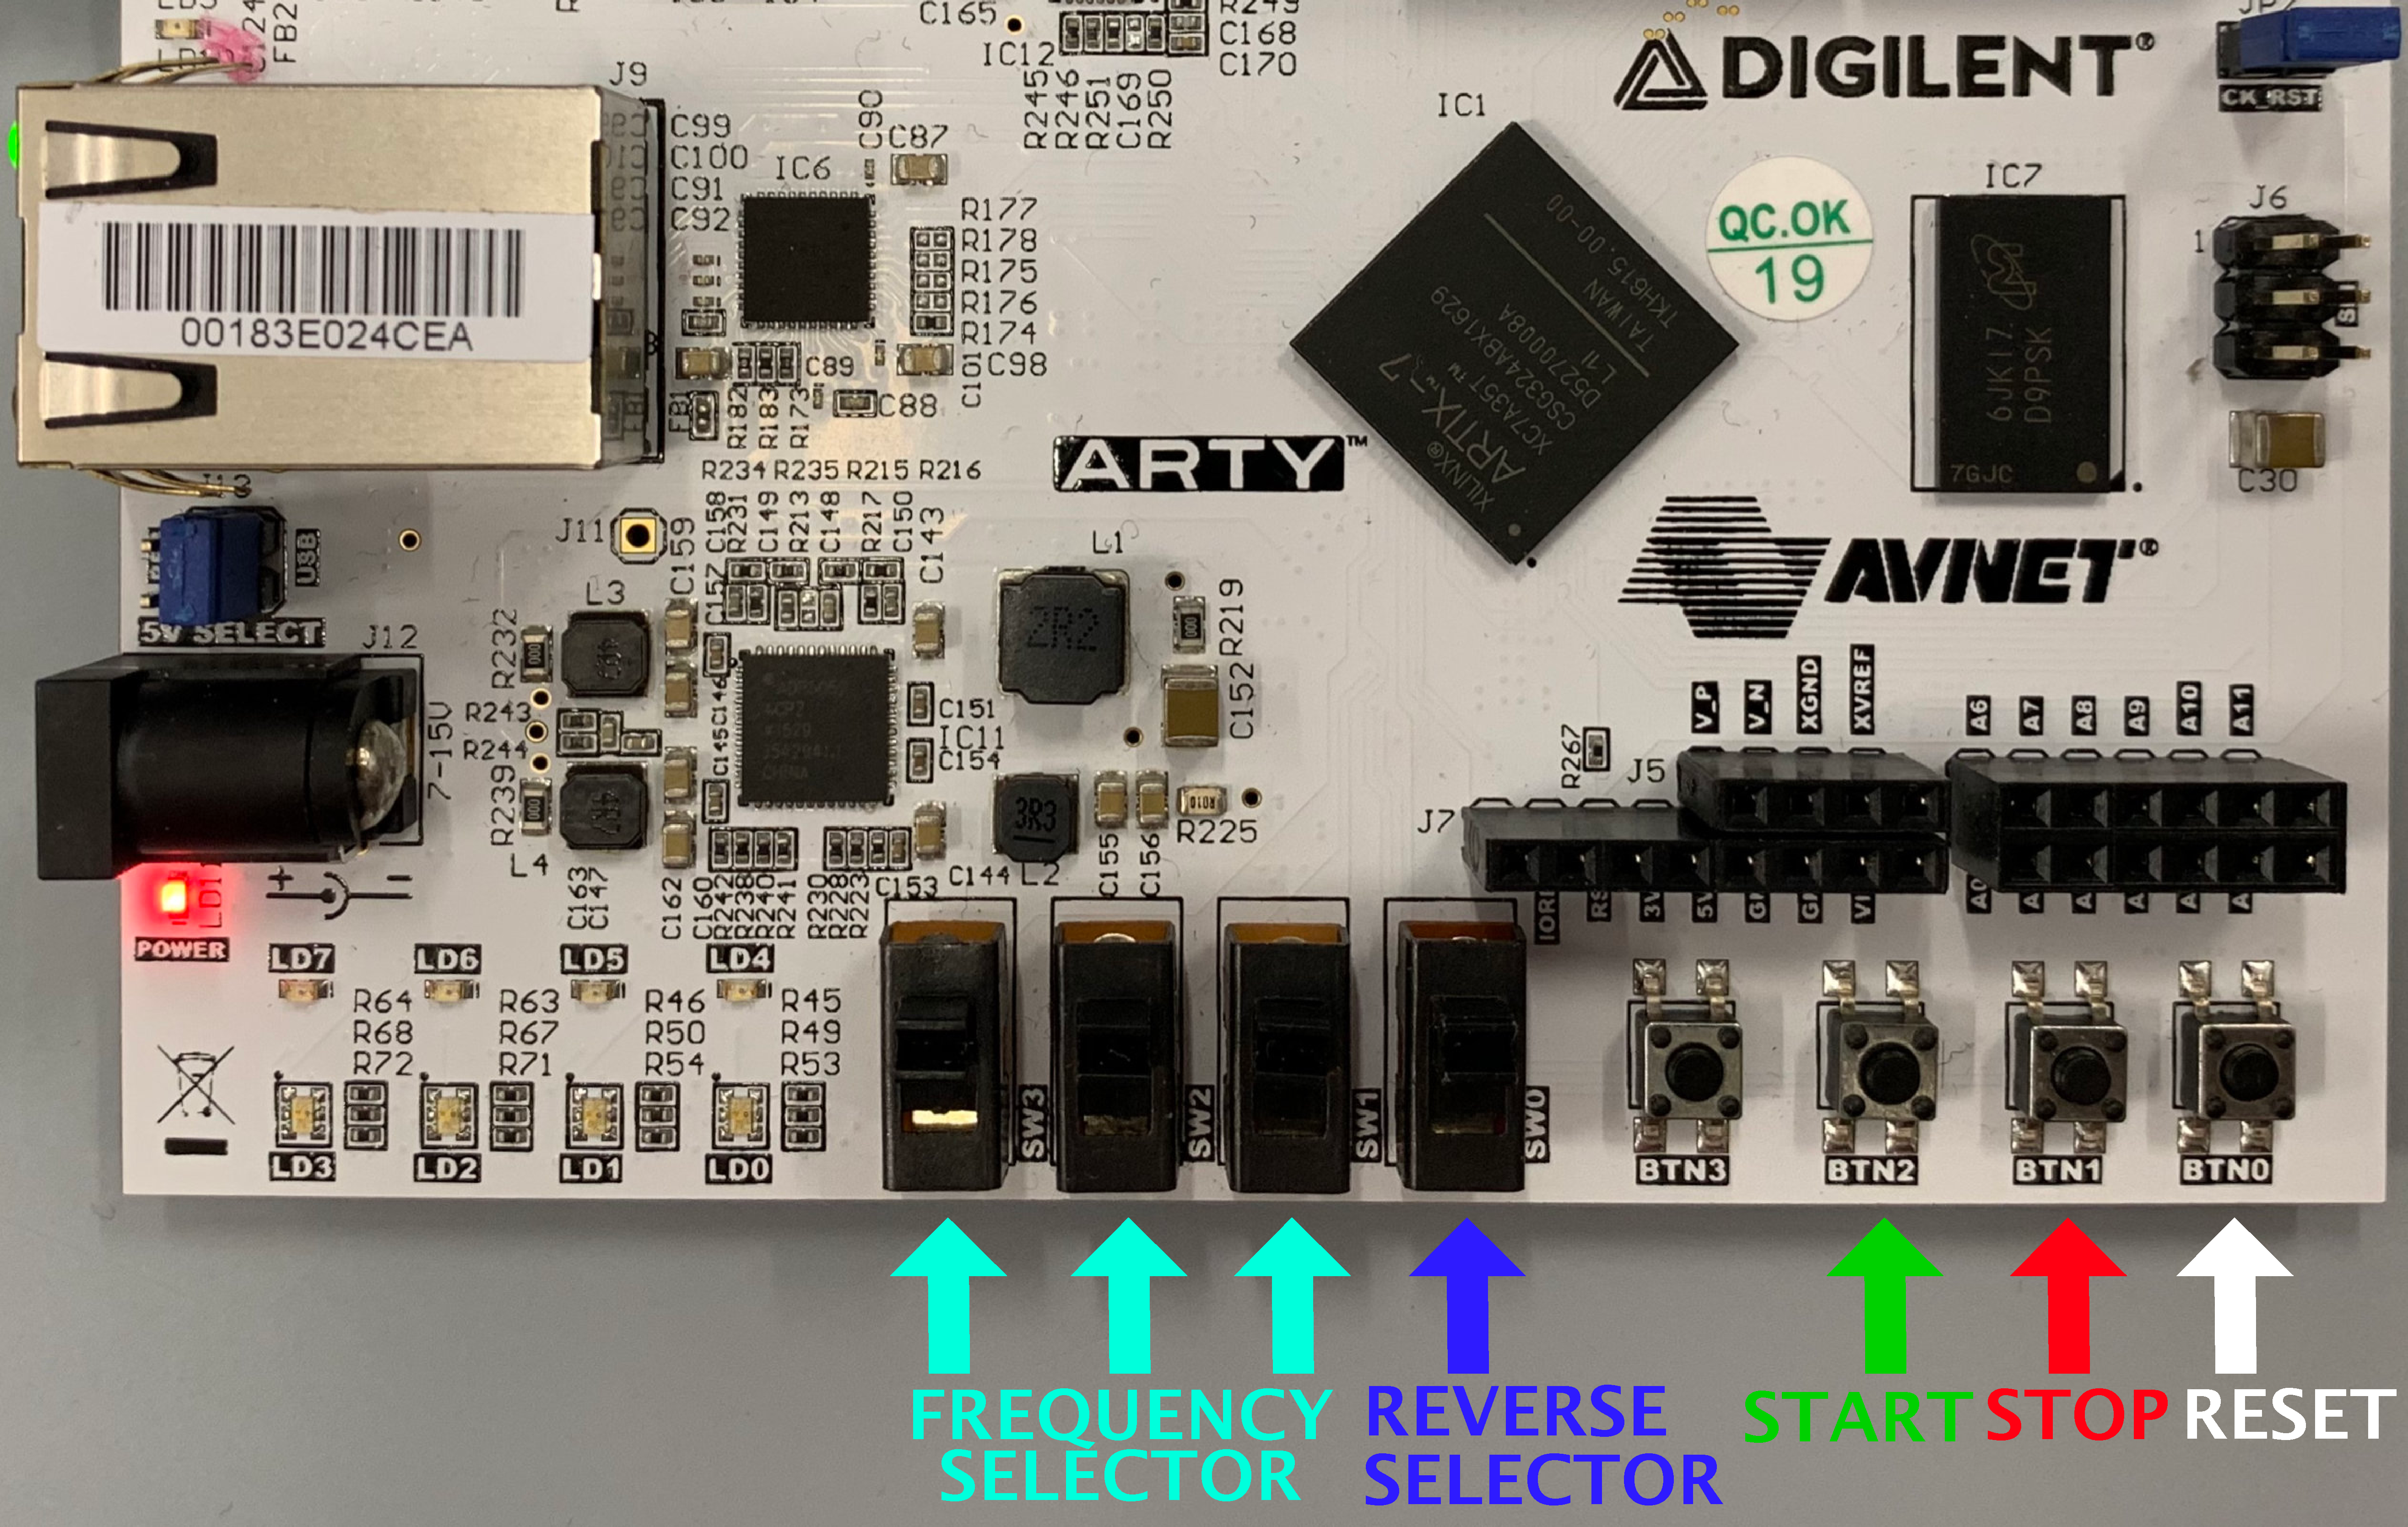
\includegraphics[width=0.7\textwidth]{../main/image/board_implementation.pdf}
\caption{\label{fig:board_implementation} Arty7 board: disposition of the functionalities.}
\end{figure}


\clearpage
\subsection{Counter}
The code implementation is constituted by four main processes. The first two processes ({\footnotesize\texttt{p\_cnt}} and {\footnotesize\texttt{p\_slw\_cnt}}) are used to implement the counter.

First of all, the clock has been used to increase the value of a vector of 28 bits ({\footnotesize\texttt{counter}}) each time the clock signal shows a rising edge, as in process {\footnotesize\texttt{p\_cnt}} (Listing \ref{lst:p_cnt}).

\begin{lstlisting}[style=vhdl,label={lst:p_cnt},caption={{\footnotesize\texttt{p\_cnt}} process.}]
p_cnt : process(clk,rst,sel_in) is
    begin
    if rst = '1' then
        counter <= (others => '0');
    end if;
    if rising_edge(clk) then
        counter <= counter +1;
    end if;
end process;\end{lstlisting}

Then, since the speed of the embedded clock is too fast, it has been slowed down in the process {\footnotesize\texttt{p\_swl\_cnt}} (Listing \ref{lst:p_slw_cnt}) by creating a slow clock signal {\footnotesize\texttt{slow\_clk}} and taking the \(i^\text{th}\) bit {\footnotesize\texttt{slow\_clk <= counter(i)}}, where the value of \(i\) is determined by the frequency selector.
The slow clock signal has eventually been used to update the {\footnotesize\texttt{slow\_counter}} signal, which reflects the four bit display counter that will be mapped to the LEDs.

\begin{lstlisting}[style=vhdl,label={lst:p_slw_cnt},caption={{\footnotesize\texttt{p\_slw\_cnt}} process.}]
p_slw_cnt : process(clk,rst,frz,slow_clk,sel_in,state) is
    begin
    if rst = '1' then
        slow_counter <= (others => '0');
    end if;
    if rising_edge(clk) then
        slow_clk_p <= slow_clk;
        if state = '0' then
            if slow_clk = '1' and slow_clk_p = '0' then
                if sel_in(0) = '0' then
                    slow_counter <= slow_counter + 1;
                elsif sel_in(0) = '1' then
                    slow_counter <= slow_counter - 1;
                end if;
            end if;
        end if;
    end if;
end process;\end{lstlisting}



\subsection{FREQUENCY and REVERSE SELECTOR}
In order to select manually the speed of the display counter, the value of the \(i^\text{th}\) element of the vector {\footnotesize\texttt{counter}} is chosen based on the values of the three elements of {\footnotesize\texttt{sel}} vector. The ladder reflects the status of the three switches. It is implemented in the {\footnotesize\texttt{speed}} process (Listing \ref{lst:speed}).
Moreover, in order to reverse the counter, {\footnotesize\texttt{slow\_counter}} is updated forward \( (+1)\) or backward \((-1)\) based on the position of a fourth switch as shown in process {\footnotesize\texttt{p\_slw\_cnt}} (Listing \ref{lst:p_slw_cnt}).

\begin{lstlisting}[style=vhdl,label={lst:speed},caption={{\footnotesize\texttt{speed}} process.}]
speed : process(clk,rst,slow_clk,sel) is
    begin
    case sel is
        when "000" => slow_clk <= counter(27);
        when "001" => slow_clk <= counter(26);
        when "010" => slow_clk <= counter(25);
        when "011" => slow_clk <= counter(24);
        when "100" => slow_clk <= counter(23);
        when "101" => slow_clk <= counter(22);
        when "110" => slow_clk <= counter(21);
        when "111" => slow_clk <= counter(20);
        when others => null;
    end case;
end process;\end{lstlisting}



\subsection{START, STOP and RESET}
In details, when START button is pressed and then released the board starts counting, when STOP button is pressed and released the counter stops and the LEDs freeze. Finally, when RESET button is pressed and released, the counter goes to zero and stops at the same time.



START and STOP button have been implemented in the process {\footnotesize\texttt{btn\_state}} (Listing \ref{lst:btn_state}), where a variable {\footnotesize\texttt{state}} is set to ‘1’ if STOP button is pressed, while it is set to ‘0’ if START is pressed.
In the process {\footnotesize\texttt{p\_slw\_cnt}}, previously described in Listing \ref{lst:p_slw_cnt}, the update of {\footnotesize\texttt{slow\_counter}} happens only if {\footnotesize\texttt{state}} is set to ‘0’. Instead, RESET button, besides setting {\footnotesize\texttt{state}} to ‘1’ in order to stop the counter, sets {\footnotesize\texttt{counter}} and {\footnotesize\texttt{slow\_counter}} to ‘0’.

\begin{lstlisting}[style=vhdl,label={lst:btn_state},caption={{\footnotesize\texttt{btn\_state}} process.}]
btn_state : process(clk,rst,frz,start,slow_clk,sel_in,state) is
    begin
    if rising_edge(clk) then
        if start = '1' then
            state <= '0';
        elsif frz = '1' then
            state <= '1';
        elsif rst = '1' then
            state <= '1';
        end if;
    end if;
end process;\end{lstlisting}





\section{Simulation}
To be sure of the correct behaviour of the counter, we perform a behavioural simulation on Vivado, where the unit under test is {\footnotesize\texttt{cnt}} (Listing \ref{lst:uut}).

\begin{lstlisting}[style=vhdl,label={lst:uut},caption={Unit under test {\footnotesize\texttt{cnt}}.}]
uut : cnt port map (clk       => clk,
                    sel_in(0) => rev,
                    sel_in(1) => sel(0),
                    sel_in(2) => sel(1),
                    sel_in(3) => sel(2),
                    y_out     => led_out,
                    frz       => btn_frz,
                    start     => btn_start,
                    rst       => btn_rst);
\end{lstlisting}


First of all, we fix the simulation time to \( \SI{10}{\mu s} \). To visualize the behaviour of the counter in that time scale, we set a proper higher frequency of the counter for the whole time of the simulation. 
Then we define a clock signal consisting in a square wave of period $\SI{10}{\ns}$, whose transitions are implemented in {\footnotesize\texttt{p\_clk}} process (Listing \ref{lst:sim_clk}).


\begin{lstlisting}[style=vhdl,label={lst:sim_clk},caption={{\footnotesize\texttt{p\_clk}} process.}]
p_clk: process
begin
    clk <= '0'; wait for 5 ns;
    clk <= '1'; wait for 5 ns;
end process;\end{lstlisting}


Afterwards, we simulate the following routine in {\footnotesize\texttt{p\_start}} process (Listing \ref{lst:sim_pstart}):
\begin{itemize}
    \item the RESET button is pressed for $\SI{50}{\ns}$ and then released;
    \item after $\SI{50}{\ns}$, START button is pressed for $\SI{50}{\ns}$ and released;
    \item after $\SI{1200}{\ns}$, the STOP button is pressed and released after $\SI{50}{\ns}$.
\end{itemize}


\begin{lstlisting}[style=vhdl,label={lst:sim_pstart},caption={{\footnotesize\texttt{p\_start}} process.}]
p_start: process
begin
    btn_rst   <= '1'; wait for 50 ns;
    btn_rst   <= '0'; wait for 50 ns;
    btn_start <= '1'; wait for 50 ns;
    btn_start <= '0'; wait for 1200 ns;
    btn_frz   <= '1'; wait for 50 ns;
    btn_frz   <= '0'; wait for 50 ns;
end process;\end{lstlisting}

In Figure \ref{fig:sim_1} the results of the simulation are showed. The signal {\footnotesize\texttt{led\_out}} carries the value of the counter at a certain time. In this way we can see that the counter is working correctly, as well as the START, STOP and RESET functionalities.


\begin{figure}[H]
\centering
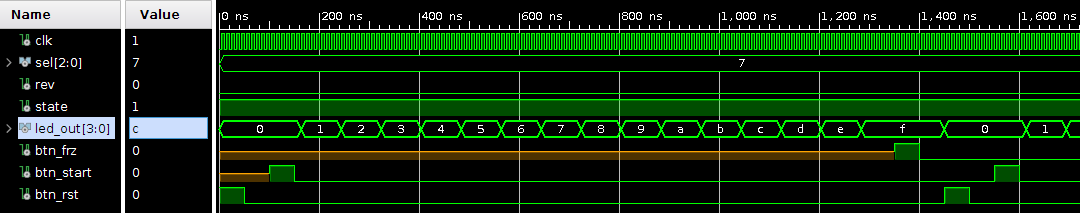
\includegraphics[width=1\textwidth]{../main/image/sim_2.png}
\caption{\label{fig:sim_1} Vivado simulation of FPGA Stopwatch.}
\end{figure}





\section{Conclusions}
This assignment presents the design of a FPGA-based Stopwatch with START, STOP and RESET functionalities.
A behavioral validation testbench has been developed and has been used to confirm a proper behaviour without glitches.
Afterwards, the system has been experimentally validated on Arty7 board with success.


\end{document}
